% vim: set ft=plaintex:

\documentclass[]{article}
\usepackage{showlabels}

\usepackage[margin=1in]{geometry}
\usepackage{fancyhdr}
\pagestyle{fancy}

\usepackage{amsmath}
\usepackage{mathtools}
\usepackage{amsfonts}
\usepackage{amssymb}
\usepackage{bbm}

\usepackage{braket}
\usepackage[bold]{hhtensor}
\usepackage{cancel}

\usepackage{amsthm}

% load thmtools but fix "proof proof" bug with thmbox
\usepackage{letltxmacro}
\LetLtxMacro\amsproof\proof
\LetLtxMacro\amsendproof\endproof

\usepackage{thmtools}

\AtBeginDocument{%
  \LetLtxMacro\proof\amsproof
  \LetLtxMacro\endproof\amsendproof
}

\usepackage{nameref,hyperref}
\usepackage[capitalize]{cleveref}

\usepackage{natbib}
\bibliographystyle{humannat}
\usepackage[nottoc]{tocbibind}
\usepackage[toc,page]{appendix}


\usepackage{algorithm2e}
\usepackage{booktabs}
\usepackage{enumitem}
\usepackage{float}
\usepackage{graphicx}
\usepackage[all]{xy}

\usepackage{comment}
\usepackage{todonotes}

% bold \emph
\let\emph\relax
\DeclareTextFontCommand{\emph}{\bfseries\em}

\declaretheorem[thmbox=M]{theorem}
\declaretheorem[thmbox=M,sibling=theorem]{proposition}
\declaretheorem[thmbox=M,sibling=theorem]{lemma}
\declaretheorem[thmbox=M,sibling=theorem]{corollary}
\declaretheorem[thmbox=M,sibling=theorem]{conjecture}
\declaretheorem[
    thmbox={style=M,bodystyle=\normalfont},
    sibling=theorem,
]{definition}
\declaretheorem[
    thmbox={style=M,bodystyle=\normalfont},
    sibling=theorem,
]{example}
\declaretheorem[style=remark,sibling=theorem]{remark}


\makeatletter
\newcommand{\myref}[1]{\cref{#1}\mynameref{#1}{\csname r@#1\endcsname}}
\newcommand{\Myref}[1]{\Cref{#1}\mynameref{#1}{\csname r@#1\endcsname}}
\def\mynameref#1#2{%
  \begingroup
    \edef\@mytxt{#2}%
    \edef\@mytst{\expandafter\@thirdoffive\@mytxt}%
    \ifx\@mytst\empty\else
    \space(\nameref{#1})\fi
  \endgroup
}
\makeatother

\newcommand{\simiid}{\overset{\text{iid}}{\sim}}
\newcommand{\eps}{\varepsilon}
\newcommand{\Rad}{\text{Rad}}


\newcommand{\NN}{\mathbb{N}}
\newcommand{\ZZ}{\mathbb{Z}}
\newcommand{\CC}{\mathbb{C}}
\newcommand{\RR}{\mathbb{R}}
\newcommand{\TT}{\mathbb{T}}
\newcommand{\ind}{\mathbbm{1}}
\newcommand{\fm}{\mathfrak{m}}

\newcommand{\cA}{\mathcal{A}}
\newcommand{\cB}{\mathcal{B}}
\newcommand{\cD}{\mathcal{D}}
\newcommand{\cE}{\mathcal{E}}
\newcommand{\cG}{\mathcal{G}}
\newcommand{\cH}{\mathcal{H}}
\newcommand{\cL}{\mathcal{L}}
\newcommand{\cN}{\mathcal{N}}
\newcommand{\cF}{\mathcal{F}}
\newcommand{\cK}{\mathcal{K}}
\newcommand{\cS}{\mathcal{S}}
\newcommand{\cU}{\mathcal{U}}
\newcommand{\cX}{\mathcal{X}}

\newcommand{\mX}{\matr{X}}
\newcommand{\mY}{\matr{Y}}
\newcommand{\mA}{\matr{A}}
\newcommand{\mB}{\matr{B}}
\newcommand{\mD}{\matr{D}}
\newcommand{\mI}{\matr{I}}
\newcommand{\mK}{\matr{K}}
\newcommand{\mL}{\matr{L}}
\newcommand{\mM}{\matr{M}}
\newcommand{\mP}{\matr{P}}
\newcommand{\mQ}{\matr{Q}}
\newcommand{\mS}{\matr{S}}
\newcommand{\mU}{\matr{U}}
\newcommand{\mV}{\matr{V}}
\newcommand{\mZ}{\matr{Z}}
\newcommand{\mSigma}{\matr{\Sigma}}
\newcommand{\mLambda}{\matr{\Lambda}}
\newcommand{\va}{\vec{a}}
\newcommand{\vb}{\vec{b}}
\newcommand{\vc}{\vec{c}}
\newcommand{\vf}{\vec{f}}
\newcommand{\vg}{\vec{g}}
\newcommand{\vk}{\vec{k}}
\newcommand{\vmu}{\vec{\mu}}
\newcommand{\vp}{\vec{p}}
\newcommand{\vq}{\vec{q}}
\newcommand{\vu}{\vec{u}}
\newcommand{\vw}{\vec{w}}
\newcommand{\vx}{\vec{x}}
\newcommand{\vy}{\vec{y}}
\newcommand{\vz}{\vec{z}}
\newcommand{\vbeta}{\vec{\beta}}
\newcommand{\vsigma}{\vec{\sigma}}
\newcommand{\vxi}{\vec{\xi}}


\DeclareMathOperator{\id}{id}
\DeclareMathOperator{\im}{im}
\DeclareMathOperator{\Ball}{Ball}
\DeclareMathOperator{\Cov}{Cov}
\DeclareMathOperator{\argmax}{argmax}
\DeclareMathOperator{\argmin}{argmin}
\DeclareMathOperator{\diag}{diag}
\DeclareMathOperator{\Var}{Var}
\DeclareMathOperator{\Tr}{Tr}
\DeclareMathOperator{\rank}{rank}
\DeclareMathOperator{\adj}{adj}
\DeclareMathOperator{\TV}{TV}
\DeclareMathOperator{\Vol}{Vol}



\newcommand{\ex}{\mathbb{E}}



\begin{document}

\title{EE290 Course Notes}
\author{Feynman Liang\thanks{\texttt{feynman@berkeley.edu}} \\ Department of Statistics, UC Berkeley}
\date{Last updated: \today}

\maketitle

\tableofcontents


\begin{comment}
\end{comment}

\section{9/5/2019}

\subsection{Results from random matrix theory}

Today we consider random matrices $Z = (Z_{ij}) \in \RR^{n \times n}$.
IID matrix ensemble is when $Z_{ij} \sim P$ are drawn IID, and the
Gaussian Orthogonal Ensemble (GOE) has $Z_{ii} \sim N(0,2)$
and $Z_{ij} = Z_{ji} \sim N(0,1)$ for $i \neq j$.

By convention, normalize and center so $\ex Z_{ij} = 0$ and $\ex Z_{ij}^2 = 1$.

\textbf{Intuition}: $\|Z\|_{op} \leq C \sqrt{n}$ with high probability.

Consider Gaussian orthogonal ensemble matrix: $Z_{ij} \sim N(0,1)$ and $Z_{ii}
\sim N(0,2)$. View $Z = \begin{bmatrix} Z_1, \ldots, Z_n \end{bmatrix}$
with $Z_i \sim N(0, I_n)$. Then
\begin{align}
  \ex \|Z_1\|_2^2 &= \ex[ \sum_{i=1}^n Z_{i1}^2 ] = n \\
  Z_1^\top Z_2 &= \sum_{i=1}^n Z_{i1} Z_{i2} \\
  \ex Z_1^\top Z_2 &= 0 \\
  \ex (Z_1^\top Z_2)^2 &= n \\
  \lvert Z_1^\top Z_2\rvert &\sim \sqrt{n} \\
  \frac{Z_1^\top Z_2}{\|Z_1\| \|Z_2\|} &\sim \frac{1}{\sqrt{n}}
\end{align}

\begin{theorem}[\cite{latala2006estimates}]
  \begin{align}
    \sup_i \sum_{j=1}^n \ex \lvert Z_{ij} \rvert^2 &\leq k^2 n \\
    \sup_j \sum_{i=1}^n \ex \lvert Z_{ij} \rvert^2 &\leq k^2 n
  \end{align}
  Fourth moment bound
  \begin{align}
    \sum_{i=1}^n \sum_{j=1}^n \ex\lvert Z_{ij}\rvert^4 \leq k^4 n^2
  \end{align}

  Then $\ex \|Z\|_{op} = O(k \sqrt{n})$
\end{theorem}

\subsection{Gaussian Orthogonal Ensemble}

$\|Z\|_{op} = \sigma_{max} = \max_{\|v\|=1} v^\top Z v$

For any fixed $v \in S^{n-1}$, we have a Gaussian tail bound
\begin{align}
  v^\top Z v
  &= \sum_i Z_{ii} v_i + \sum_{i < j} 2 Z_{ij} v_i v_j \\
  &= N(0, \sum_i v_i^4 + \sum_{i < j} 4 v_i^2 v_j^2 ) \\
  \Pr(\lvert v^\top Z v \rvert > t) &\leq 2 e^{-t^2 / 4}
\end{align}
Using an $\epsilon$-net, can find a set of vectors $V_{\epsilon}$ such that
\begin{align}
  \max_{v \in V_\epsilon} \lvert v^\top Z v \rvert
  &\geq (1 - 2 \epsilon) \max_{\lvert v \rvert = 1} \lvert z^\top Z v \rvert \geq (1 - 2 \epsilon) t
  \label{eq:eig-eps-net-lb}
\end{align}
Then by a union bound
\begin{align}
  \Pr[ \|Z\|_{op} \geq t ]
  &\leq \Pr[ \max_{v \in V_\epsilon} \lvert v^\top Z v \rvert \geq (1 - 2\epsilon) t ] \\
  &\leq \sum_{v \in V_\epsilon} \Pr[ \lvert v^\top Z v \rvert \geq (1 - 2\epsilon) t ] \\
  &\leq 2 \lvert V \rvert e^{-\frac{1}{4}(1 - 2 \epsilon)^2 t^2} \leq \delta
\end{align}
If $\lvert V \rvert \leq c^n$, then
\begin{align}
  e^{c (n - c t^2)} &\leq e^{\log \delta} \\
  \log \frac{1}{\delta} \leq c t^2 - n &\implies t \geq \sqrt{n + \log \frac{1}{\delta}}
\end{align}

Intuition: when dealing with infinite dimensional maximization (Rayleigh quotient for eigenvalue problem),
can pass to $\epsilon$-net for cardinality bboud.

\begin{definition}[Covering]
  $V \subset S^{n-1}$ is called an $\epsilon$-net if $\forall u \in S^{n-1}$,
  $\exists v \in V$ such that $\|u - v\|_2 \leq \epsilon$.
\end{definition}

\begin{theorem}
  $\epsilon$-net yields \cref{eq:eig-eps-net-lb}
\end{theorem}

\begin{definition}[Packing]
  For $A \subset \RR^d$, $V = \{v_i\}_{i=1}^n \subset A$ is an
  $\epsilon$-packing if $\forall i \neq jJ$, $\| v_i - v_j\|_2 \geq \epsilon$.
\end{definition}

\begin{theorem}
  Maximal $\epsilon$-packing is an $\epsilon$-net.
\end{theorem}

Hence, we can lower bound the packing number (size of largest packing)
by the covering number (size of the smallest covering).
The following result gives an (obvious?) upper bound:

\begin{lemma}[Volume ratio]
  For any $\epsilon$-packing $V \subset A$,
  \begin{align}
    \lvert V \rvert
    \leq \frac{\text{Vol}(A + \frac{\epsilon}{2} B)}{\text{Vol}(\frac{\epsilon}{2} B)}
  \end{align}
  where $B = \{x : \|x\|_2 \leq 1\}$.
\end{lemma}


Why is the diagonal not important? Let $A = \diag(Z)$. Then we have
\begin{align}
  \|Z - A\|_{op}
  &\leq \|Z\|_{op} + \|A\|_{op} \\
  \max_{x \in S^{n-1}} \| A x \| &= \max_i \lvert Z_{ii} \rvert = O(\sqrt{2 \log n})
\end{align}
So the diagonal term $\|A\|_{op}$ is an order of magnitude
smaller that $\|Z\|_{op}$.

\begin{example}[Planted clique]
    Let $G \sim G(1/2, n, k)$. In other words,
    generate an Erd\"os-Renyi random graph from $G(n, 1/2)$ and then
    randomly choose a set $K \subset [n]$ connect together to form a clique.
    
    Goal: find $K$ given $G$.
    
    \begin{theorem}[\cite{alon1998finding}]
      For any $c$, $k = c \sqrt{n}$, then exists polytime algorithm such that
      it returns $\hat{K}$ with $P(\hat{K} = K) \to 1$.
    \end{theorem}
    
    Let the adjacency matrix $A_{ij} = \begin{cases}
        1 & (i,j) \in K \\
        \text{Bern}(1/2) & i \not\in K\text{ or }j \not\in K, i \neq j \\
        0 & i = j
    \end{cases}$ and define $W_{ij} = \begin{cases}
        2 A_{ij} - 1 & i \neq j \\
        0 & i = j
    \end{cases}$
    
    \begin{enumerate}
        \item Find top eigenvector $u$ of $W$
        \item Let $\tilde{K}$ index the $k$ largest coordinates $\lvert u_i \rvert$
        \item  Thresholding
        \begin{align}
            \hat{K} &= \left\{v \in [n] : d_{\tilde{K}}(v) \geq \frac{3k}{4} \right\} \\
            d_{\tilde{K}}(v) &= \sum_{j \in \tilde{K}} \ind\{(j,v) \text{ connected}\}
        \end{align}
    \end{enumerate}
    
    
    Goal: show $\lvert \tilde{K} \cap K \rvert \geq (1 - \epsilon) k$ whp.
    
    Note that $\ex[W] \eqqcolon 1_k 1_k^\top - \diag(1_k)$ consists of $1$s in $K \times K$
    and $0$ everywhere else. Let
    \begin{align}
        W^* &= 1_k 1_k^\top \\
        v &= \frac{1}{\sqrt{k}} 1_k \\
    \end{align}
    Notice thresholding over $v$ exactly recovers $K$, so we want the top
    eigenvector $u$ of $W$ to be close to $v$. By Davis-Kahan,
    \begin{align}
        \min_{s \in \{\pm 1\}} \|u + s v\|_2
        &\leq \frac{\|W - W^*\|_{op}}{\lambda_1(W^*) - \lambda_2(W^*)}
    \end{align}
    Note $\lambda_1(W^*) = k$.
    Suppose extrema attained at $s=-1$, then
    \begin{align}
        \|W - W^*\|_{op} 
        \leq \|W - \ex W\| + \underbrace{\|\ex W - W^*\|}_{=\|\diag 1_k\| = 1}
        \leq c \sqrt{n} + 1
    \end{align}
    
    By Weyl's inequality
    \begin{align}
        \lvert \lambda_2(W) \rvert
        = \lvert \lambda_2(W^*) - \lambda_2(W) \rvert
        \leq \|W^* - W\|_{op}
        \leq c \sqrt{n} + 1
    \end{align}
    Finally
    \begin{align}
        \|u - v\|_2 
        \leq \frac{c \sqrt{n} + 1}{c \sqrt{n} - (c \sqrt{n} + 1)}
        \leq \epsilon
    \end{align}
\end{example}

NOTE: when you have bounded fourth moments, the rate is always $n^{-1/2}$! Deep result.

\section{9/10/2019}

Recall the planted clique from \cite{alon1998finding}: $G \sim G(1/2, n, k)$
is a random graph on $V = [n]$ with some fully connected
clique $K \subset [n]$ of cardinality $\lvert K \rvert = k$.

The adjacency matrix
\begin{align}
  A_{ij} &=
  \begin{cases}
    1 &\text{if }i,j \in K \\
    \text{Bern}(1/2) &\text{$i \neq j$ ow}
  \end{cases}
\end{align}

Let
\begin{align}
    W_{ij} &= \begin{cases}
        2 A_{ij} &\text{if }i \neq j \\
        0 &\text{if }i = j
    \end{cases}
\end{align}
Algorithm 1 of \cite{alon1998finding}:
\begin{enumerate}
    \item Find top eigenvector of $W$, say $u$
    \item Let $\tilde{K}$ index the largest $k$ coordinates $\lvert u_i \rvert$
    \item Define $\hat{K} = \{ v \in V : d_{\tilde{K}}(v) \geq \frac{3 k}{4} \}$
\end{enumerate}

\begin{theorem}[\cite{alon1998finding}]
    Algorithm 1 finds $\hat{K}$ such that $\Pr[\hat{K} = K] \to 1$ as $n \to \infty$
    if $k \geq c \sqrt{n}$ for sufficiently large $c$.
\end{theorem}

\begin{proof}
    Note that $\ex A$ is:
    \begin{figure}[H]
        \centering
        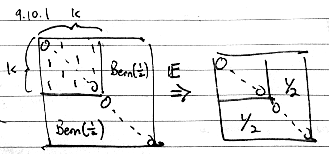
\includegraphics[width=0.6\textwidth]{figures/9-10-1.png}
        \caption{$\ex A$ has ones in the upper $k \times k$ block,
            $0$ on the diagonal, and $1/2$ everywhere else}
    \end{figure}
    
    From this, we can easily see that the $\ex W$ is:
    \begin{figure}[H]
        \centering
        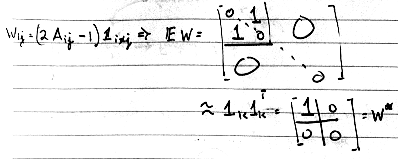
\includegraphics[width=0.6\textwidth]{figures/9-10-2.png}
        \caption{$\ex W$ differs from $W^* = 1_k 1_k^\top$ only in the upper $k$ diagonal}
    \end{figure}
    Note $\ex W = 1_K 1_K^\top - \diag(1_K) \approx 1_K 1_K^\top = W^*$, which
    is good because we have seen that ``differenes in the diagonal are asymptotically negligible.'' \todo{reference for this? 9-5 lecture}
    
    \textbf{Goal}: show $\lvert \tilde{K} \cap K \rvert \geq (1 - \eps) k$ whp, $\eps = \eps(c)$.
    
    We first show the top eigenvector of $W^*$ is close
    to $u$ (the top eigenvector of $W$).
    Let $v = \frac{1}{\sqrt{k}} 1_K$ be the top eigenvector of $W^*$.
    Note $\lambda_1(W^*) = k$.
    By Davis-Kahan
    \begin{align}
        \min_{s \in \{\pm 1\}} \|u + s v\|_2
        &\leq \frac{\|W - W^*\|_{2}}{\lambda_1(w^*) - \lambda_2(w)}
    \end{align}
    Note
    \begin{align}
        \|W - W^*\|
        &\leq \|W - \ex W\| + \|\ex W - W^* \|
        \leq c \sqrt{n} + 1
    \end{align}
    Also $\lambda_1(W^*) = k$ and
    \begin{align}
        \lvert \lambda_2(W) \rvert
        &\leq \lvert \lambda_2(W^*) - \lambda_2(W)
        \leq \|W^* - W\|
    \end{align}
    So by Weyl's inequality
    \begin{align}
        \min_{s \in \{\pm 1\}} \|u + s v\|_2
        &\leq \frac{c \sqrt{n} + 1}{ k - (c \sqrt{n} + 1)} \\
        &\leq \frac{c \sqrt{n} + 1}{c \sqrt{n} - c \sqrt{n} + 1}
        \leq \eps
    \end{align}
        
    Aside: Davis-Kahan to get bound between difference of eigenvectors in 2-norm. Open problem
    to control others.
    
    Next, if $\lvert K \rvert = k = \lvert \tilde{K} \rvert$ then
    $\lvert K \setminus \tilde{K}\rvert = \lvert \tilde{K} \setminus K \rvert$.
    
    \begin{figure}[H]
        \centering
        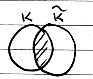
\includegraphics[width=0.2\textwidth]{figures/9-10-3.png}
        \caption{$\lvert K \rvert = \lvert \tilde{K} \rvert \implies \lvert K \setminus \tilde{K} \rvert = \lvert \tilde{K} \setminus K \rvert$ follows from elementary set theory}
    \end{figure}
    
    By definition of $v$
    \begin{align}
        \eps^2
        \geq \|u - v\|_2^2
        = \sum_{i \in K} (u_i - \frac{1}{\sqrt{k}})^2 + \sum_{i \not\in K} u_i^2
    \end{align}
    
    \begin{lemma}
        If all $\lvert u_i \rvert \leq \frac{1}{2 \sqrt{k}}$ for $i \not\in \tilde{K}$, 
        then
        \begin{align}
            \eps^2 
            \geq \sum_{i \in K \setminus \tilde{K}} (\frac{1}{\sqrt{k}} - u_i)^{2} 
            \geq \sum_{i \in K \setminus \tilde{K}} \frac{1}{4k}
        \end{align}
        This implies $\lvert K \setminus \tilde{K} \rvert \leq 4 \eps^2 k$.
    \end{lemma}
    
    \begin{lemma}
        If the condition of the previous lemma does not hold, then $\exists i \in \tilde{K}$
        with $\lvert u_i \rvert \geq \frac{1}{2 \sqrt{k}}$. Then in fact $\lvert u_i \rvert \geq \frac{1}{2 \sqrt{k}}$ for all $i \in \tilde{K}$ since
        \begin{align}
            \eps^2
            &\geq \sum_{i \in \tilde{K} \setminus K} u_i^2
            \geq \sum_{i \in \tilde{K} \setminus K} (\frac{1}{2 \sqrt{k}})^2
            = \sum_{i \in \tilde{K} \setminus K} \frac{1}{4k}
        \end{align}
        Hence $\lvert \tilde{K} \setminus K \rvert \leq 4 \eps^2 k$
    \end{lemma}
    So we have achieved our goal.
    
    To finish the proof, first assume $\|u - v\|_2 \leq \eps$.
    For $a \in K$,
    \begin{align}
        d_{\tilde{K}}(a)
        \geq d_{\tilde{K} \cap K}(a)
        = \lvert \tilde{K} \cap K \rvert - 1
        \geq (1 - \eps') k
    \end{align}
    so for $a \in K$, we will get $a \in \hat{K}$.
    
    Now if $a \not\in K$,
    \begin{align}
        d_{\tilde{K}}(a)
        \leq \underbrace{d_K(a)}_{\sim \text{Binom}(k, 1/2)} + \underbrace{\lvert \tilde{K} \setminus K \rvert}_{\leq \eps' k}
        \approx \frac{k}{2} \pm c \sqrt{k}
    \end{align}
    where $\approx$ means concentration. To be concrete,
    \begin{align}
        \Pr[\hat{K} \neq K]
        &\leq \Pr[\|u - v\|_2 \geq t]
        + \Pr[\exists a \not\in K : d_K(a) \geq (\frac{3}{4} - \eps') k] \\
        &\leq \Pr[ \|W - \ex W\| \geq c \sqrt{n} ]
        + (n - k) \Pr[B(k, 1/2) \geq (\frac{3}{4} - \eps) k] \\
        &\leq c e^{-c' n} + (n - k)
    \end{align}
    
    Where above we used the multiplicative version of Chernoff bound 
    (useful in combinatorial statistics):
    \begin{lemma}[Multiplicative Chernoff Bound]\label{lem:mult-chernoff}
        \begin{align}
            \Pr[X \geq (1 + \delta) \mu]
            &\leq \begin{cases}
                e^{-\delta^2 \mu / 3} &\delta \in [0,1] \\
                e^{-\delta \mu / 3} &\delta \geq 1
            \end{cases} \\
            \Pr[X \leq (1 - \delta) \mu]
            &\leq e^{-\delta^2 \mu / 2}
        \end{align}
    \end{lemma}
    
    As $n \to \infty$, we see that $\Pr[\hat{K} = K] \to 1$.
\end{proof}

\cref{lem:mult-chernoff} is self-normalizing: let $X = \sum_{i=1}^n X_i$ with $X_i$ independent binary
and $\mu = \ex X$. Note that after applying, the RHS does not depend on $n$ \todo{Verify}


\textbf{AKS Algorithm 2}: This algorithm is designed to handle the case when $k$ is not big enough
(recall algorithm 1 requires $k \geq c \sqrt{n}$).
Search over all $S$ with $\lvert S \rvert = C(c) = 2 \log_2 \frac{10}{c} + 2$. For each $S$:
\begin{enumerate}
    \item Define $N^*(S) = \{ v \in V : v \sim a, \forall a \in S \} \setminus S$
    \item Run Algorithm 1 on the induced subgraph (which has distribution $G(1/2, N^*(S), K-S)$),
        return $Q_S \cup S$
    \item Output if $Q_S \cup S$ is a $k$-clique
\end{enumerate}

\textbf{Intuition}: Suppose $k=0$ so there's no clique. Then $\lvert N^*(S) \rvert \sim B(n-s, 2^{-s})
\approx \frac{n-s}{2^s}$ so the total number of nodes is much smaller (by order of $2^{-s}$).
However, the number of clique nodes in $N^*(S)$ is still relatively large, $\geq k - s$.
Solving the critical equation (also for algorithm 1 \todo{Track htis down})
\begin{align}
    k - s \geq C \sqrt{\frac{n}{2^s}}
\end{align}
yields the expression for $C(c)$.


\begin{theorem}
    As long as $k \geq (2 + \eps) \log_2 n$, then exhaustive search finds $k$
    with probability $\to 1$.
\end{theorem}

\begin{proof}
    Exhaustive search will always find the clique, but it may return a clique that we didn't plant.
    So we need to guarantee there is no clique of size $(2 + \eps) \log_2 n$ in $G$ whp.
    
    For $S \subset [n]$, $\lvert S \rvert = k$,
    \begin{align}
        \Pr[S~\text{is clique}] &= \frac{1}{2^{\binom{k}{2}}} \\
        \Pr[\exists S \subset [n] : S~\text{is clique}]
        &\leq \binom{n}{k} \frac{1}{2^{\binom{k}{2}}} 
        \leq (n 2^{-(k-1)/2})^k \to 0\\
    \end{align}
    as $n \to \infty$ ($k = (2 + \eps) \log_2 n$).
\end{proof}
\section{9/12/2019}

\subsection{Planted cliques and semidefinite programming}

Recall the matrix $W$ from before, which has $1$s in the top $k \times k$ block, zero on the diagonal, and $\text{Rad}(1/2)$ RVs elsewhere.

Recall the spectral method:
\begin{align}\label{eq:9-12-orig-spec}
    \hat{u}_{spec} &= \argmax_{\substack{u \in \RR^n \\ \|u\|^2 = k}} u^\top W u
\end{align}
This needs a cleaning step, which we analyzed previously.

How did they come up with this algorithm?
Can we get more insight by analyzing htis method in a more principled framework?
Yes, through maximum likelihood!

Consider an alterantive model where within clique we have connection probability $p$ (instead of $1$) and other connections with probability $q$ (instead of $1/2$),
where $p \gg q$.
\begin{align}\label{eq:9-12-mle}
    \hat{u}_{MLE} &= \argmax_{\substack{u \in \{0,1\}^n \\ \sum_i u_i = k}} u^\top W u
\end{align}

From this, we see that the spectral method is a continuous relaxation of the
MLE integer program. To make this more precise, consider the SDP
\begin{align}\label{eq:9-12-sdp-spec}
    \hat{X}_{spec} &= \argmax_{\substack{X \succeq 0 \\ \Tr X = k}} \braket{W, X}
\end{align}
If we let $X = u u^\top$, then we automatically have $X \succeq 0$ and additionally we have $\Tr X = \|u\|_2^2$. Thus, the feasible set of
\cref{eq:9-12-orig-spec} is the same as \cref{eq:9-12-sdp-spec}.

How do we know the optima of \cref{eq:9-12-sdp-spec} is attained at a rank $1$ matrix
$X = u u^\top$? Since $X = \sum_i \lambda_i u_i u_i^\top$ ($\lambda_i \geq 0$) 
and optima are attained at extremal points, by linearity of $\braket{W,X}$ we can
put all of the weight on a single $\lambda_i$ corresponding to the top eigenvector
of $W$.

How can we get \cref{eq:9-12-sdp-spec} closer to \cref{eq:9-12-mle}? Since
\cref{eq:9-12-mle} is more constrained, we can consider adding more constraints:
\begin{align}\label{eq:9-12-mle-sdp}
    \tilde{X}_{MLE} &= \argmax_X \braket{W, X} \\
    \text{s.t. } & X \succeq 0 \\
                & \Tr X = k \\
                & 0 \leq X \leq J \quad\text{entrywise}\\
                & \braket{X, J} = k^2 \\
                & \rank(X) = 1
\end{align}
where $J = 1 1^\top$.

The solution $X = u u^\top$ where $u \in \{0,1\}^n$, where $u$
indexes the clique.

Conversely, we need to show that the feasible set coincides with \cref{eq:9-12-mle}.
If $X \succeq 0$ and $\rank X = 1$, then we can always write
$X = u u^\top$. The trace constraint now reads $k = \Tr X = \sum_i u_i^2$.
The third constraint becomes $\braket{X, J} = k^2 \implies (\sum_i u_i)^2 = k^2$.

\begin{proposition}
    The optima of \cref{eq:9-12-mle-sdp} must satisfy:
    $u_i \in [-1, 1]$, $\sum u_i^2 = k$, $(\sum_i u_i)^2 = k^2$, 
    $\{u_i\} \in \{0,1\}^n$ or $\{u_i\} \in \{0, -1\}^n$.
    
    In fact, the solution is $u = 1_k$ or $u = -1_k$.
\end{proposition}

The linear constraints in \cref{eq:9-12-mle-sdp} are fine, but the rank constraints
are difficult.
Here is an easier candidate SDP:
\begin{align}\label{eq:9-12-mle-sdp-relax}
    \hat{X}_{SDP} &= \argmax_X \braket{W, X} \\
    \text{s.t. } & X \preceq 0 \\
                 & X \geq 0 \\
                 & \Tr X = k \\
                 & \braket{X, J} = k^2
\end{align}
Notice we have dropped the rank constraint as well as the upper entrywise bound.

\begin{theorem}
    $\exists c > 0$ such that for $k \geq c \sqrt{n}$, \cref{eq:9-12-mle-sdp-relax}
    has unique maximizer $X^* = 1_k 1_k^\top$ with high probability.
\end{theorem}

\begin{proof}
    We first show $X^*$ is a maximizer.
    \begin{align}
        \braket{W, X^*} &= 1_k^\top W 1_k = k^2 - k \\
        \braket{W, X} &= \braket{W + I, X} - \Tr X \\
        \Tr(I - X) = \Tr X &\leq \braket{J, X} - \Tr(X) \\
        \underbrace{W + I \leq J}_{X \geq 0} &\implies \braket{J, X} \geq \braket{W + I, X} \\
        \therefore \Tr(I - X) = \Tr X &\leq k^2 - k
    \end{align}
    
    The harder part is uniqueness. We will develop a general technique called
    dual certificate / KKT condition.
    Write the Lagrangian for the optimization problem.
    Introduce dual variables $S \succeq 0$, $B \geq 0$,
    $\eta \in \RR$, $\lambda \in \RR$ and 
    \begin{align}
        \cL(X, S, B, \eta, \lambda)
        &= \braket{W, X} + \braket{S, X} + \braket{B, X} + \eta\left(
            k \Tr(X) + \lambda (k^2 - \braket{X, J}
        \right)
    \end{align}
    Notice
    \begin{align}
        \max_{X\text{ feas}} \braket{W, X} &= \max_X \min_{S, B, \eta, \lambda} \cL
    \end{align}
    as desired. Since $\cL$ is linear, by Sion's minimax theorem we have
    \begin{align}
        \max_X \min_{S, B, \eta, \lambda} \cL
        &= \min_{S, B, \eta, \lambda} \max_X \cL
    \end{align}
    Note $\braket{S,X} = \Tr( S^{1/2} X S^{1/2} ) \geq 0$ is non-negative.
    $\braket{B, X}$ is also trivially non-negative.
    
    \begin{lemma}\label{lem:x-star-unique-maximizer}
        The following conditions imply $X^*$ is the unique maximizer:
        \begin{enumerate}
            \item Stationarity: $W + S + B - \eta I - \lambda J = 0$ (can't improve any more)
            \item Primal/dual feasibility
            \item Complementary slackness: $\braket{S, X^*} = 0$ and $\braket{B, X^*} = 0$.
            \item Uniqueness: $\lambda_{n-1}(S) > 0$ (second smallest eigenvalue of $S$)
        \end{enumerate}
        The first three conditions are the ``KKT conditions.'' Together,
        they guarantee $X$ is a maximizer.
    \end{lemma}
    
    \begin{proof}[Proof of \cref{lem:x-star-unique-maximizer}]
        \textbf{$X^*$ is a maximizer}: for feasible variables
        \begin{align}
            \braket{W, X} &\leq \cL(X, S, B, \eta, \lambda) &&\text{feasible} \\
            &= \cL(X^*, S, B, \eta, \lambda) &&\text{stationarity} \\
            &= \braket{W, X^*} &&\text{comp. slackness}
        \end{align}
        
        \textbf{Uniqueness}: Suppose $X'$ satisfies $\braket{W, X'} = \braket{W, X^*}$.
        Then $\braket{S, X'} = 0$, and
        $\braket{S, X^*} = 0 \implies 1_k^\top S 1_k = 0 \implies S 1_k = 0$.
        In other words, $1_k$ is an eignevector with eigenvalue $0$ for $S$.
        But condition (4) means that $1_k$ is the only eigenvector with eigenvalue
        $0$, hence $X' = c X^*$ for some $c \in \RR$. But by the
        constrant $\Tr X = k$, we must have $X' = X^*$.
    \end{proof}
    
    Hence, if we can find $(S, B, \eta, \lambda)$ satisfying \cref{lem:x-star-unique-maximizer}, then we have a certificate that
    $X^*$ is the unique maximizer.
    
    But how can we find this certificate? It's hard in general, but in this
    case we have an explicit construction.
    \begin{align}
        B \geq 0, \quad \eta \in \RR, \quad \lambda \in \RR \\
        S = \eta I + \lambda J - B - W \succeq 0 \\
        S 1_k = 0, \quad \braket{B, X^*} = 0, \quad \lambda_{n-1}(S) > 0 \label{eq:9-12-star}
    \end{align}
    \begin{align}
        S 1_k = 0 \implies \eta I_k + \lambda k 1 = B 1_k + W 1_k
    \end{align}
    $X^* = 1_k 1_k^\top$. Since we want $\braket{B, X^*} = 0$, we want
    $B_{ij} = 0$ for $(i,j) \in K \times K$.
    This implies that $(B 1_k)i = 0$ for $i \in K$.
    Let $y = W 1_k$.
    
    $i$th entry, $i \in K$, of \cref{eq:9-12-star} implies $\eta + k \lambda = (B 1_k)_i + y_i = k-1$. Then, choose $\eta = k - 1 - k \lambda$
    
    Now for $i \not\in K$, \cref{eq:9-12-star} implies $\lambda k = (B 1_k)_i + y_i$.
    Construct $B = 1_k b^\top + b 1_k^\top$ for some $b \in \RR^n$ such
    that $b_i = 0$ for $i \in K$.
    Then $B 1_k = k b$.
    
    Fig 9.12.1
    
    $b_i = \lambda - \frac{y_i}{k}$ for all $i \not\in k$.
    Check $B \geq 0 \implies b_i \geq 0$. Since $\lambda \geq \frac{y_i}{k}$ for all
    $i \in K$, $\lambda \geq \max_{i \not\in K} \frac{y_i}{k}$.
    $y_i = W 1_k$ which is a sum of $\text{Rad}(1/2)$ RVs, so 
    by concentration for some $\lambda \geq c$ this is satisfied whp.
    
    For the last part, we need to show $x^\top S x > 0$ for all $x$ such that
    $x^\top 1_k = 0$. The exact formula for $S$ is 
    \begin{align}
        S 
        &= \eta + \underbrace{\lambda x^\top J x}_{\geq O(\sqrt{n})} - \underbrace{x^\top B x}_{=0} - \underbrace{x^\top W x}_{\geq O(\sqrt{n})} \\
        &\geq \frac{k}{2} - 1 - x^\top \ex[W] x - \|W - \ex W\|_{op} \\
        &\geq 0 &&\text{for suff large $k$}
    \end{align}
\end{proof}
\section{9/17/2019}

\subsection{Logistics}

HW1 releasted

\subsection{Primal method for SDP}

Planted Clique model $G(1/2, n, k)$.

\begin{align}
  \hat{X}_{SDP} &= \argmax_X \braket{W,X} \\
  st~X &\succeq 0 \\
  X &\geq 0 \\
  \Tr(X) &= k \\
  \braket{X, J} &= k^2
\end{align}
where $J = 1 1^\top$ and $W_{ij} = \ind\{i=j\} 2 A_{ij} - 1$.
Last time we proved (using a dual certificate approach)
\begin{theorem}
  If $k \geq c \sqrt{n}$ for a large enough $c$, then $X^* = 1_k 1_k^\top$
  is the unique maximizer.
\end{theorem}

Today we will consider a primal approach.

\textbf{Round up suffices}: Suppose we find $X$ such that
$\braket{W, X} \geq (1 - \eps) \braket{W, X^*}$. Let
$\hat{X}_{ij} = \ind\{X_{ij} > 1/2\}$.

\begin{theorem}
  If $\eps \lesssim \frac{c_0 \sqrt{n}}{k^3}$ for sufficiently small $c_0 < 0$,
  then $\hat{X} = X^*$ whp.
\end{theorem}

\begin{proof}
  Suppose $\hat{X} \neq X^*$. Then either:

  $\exists (i_0, j_0) \in K \times K$
  such that $X_{i_0, j_0}^* = 1$ and $X_{i_0, j_0} \leq \frac{1}{2}$,
  or

  $\exists (i_1, j_1) \not\in K \times K$ such that $X_{i_1,j_1}^* = 0$
  and $X_{i_1,j_1} > \frac{1}{2}$.

  In both acses, $\|X - X^*\|_F \geq \frac{1}{2}$.

  Also, we previously showed that the global optimum $\braket{W, X^*} = k^2 - k$
  because even though $W$ is random, inner product with $X^*$ grabs the upper left
  $K \times K$ corner where $W$ is deterministic.

  Recall the KKT condition: $S \succeq 0$, $S 1_K = 0$, $B \geq 0$, $\eta, \lambda \in \RR$,
  $\lambda_{n-1}(S) \geq c_2 \sqrt{n}$. ALso
  \begin{align}
    \braket{W, X^*} - \braket{W, X} &= \braket{S, X} + \braket{B, X} \eqqcolon \delta
  \end{align}
  because last class we had
  \begin{align}
    \braket{W, X}
    &\leq L(X, S, B, \eta, \lambda) \\
    &= \braket{W, X} + \braket{S, X} + \braket{B, X} + \eta(k - \Tr X) + \lambda (k^2 - \braket{X,J}) \\
    &= \braket{W, X^*}
  \end{align}

  We already knew $u = \frac{1}{\sqrt{k}} 1_k$ eigenvector of $S$ corresponding to $\lambda_n(S) = 0$
  (KKT complementary slackness tells us that $S u = 0$). This gives the matrix
  inequality
  \begin{align}
    S \succeq \lambda_{n-1}(S)(I - U U^\top)
  \end{align}
  Since we previously have a bound on $\braket{S,X}$, to look for a sandwich inequality
  we consider taking an inner product with $X$
  \begin{align}
    \braket{S, X}
    &\geq c_2 \sqrt{n} \braket{X, I - X^* / k}
    =  c_2 \sqrt{n} \braket{X, I} - c_2 \frac{\sqrt{n}}{k} \braket{X, X^*} \\
    \braket{X, X^*} &\geq k^2 - \frac{k \delta}{c_2 \sqrt{n}}
  \end{align}
  Where we used the upper bound
  \begin{align}
    \delta \geq \braket{S, X}
  \end{align}
  This gives a bound on a cross term in the Frobenius norm expansion
  \begin{align}
    \|X - X^*\|_F^2
    &= \|X\|_F^2 + \|X^*\|_F^2 - 2 \braket{X, X^*} \\
    \|X^*\|_F^2 &= \|1_k 1_k^\top\|_F^2 = k^2 \\
    \|X\|_F^2 &\leq \|X\|_\ast^2 = k^2 \\
    \therefore \|X - X^*\|_F^2
              &\leq k^2 + k^2 - 2 \left(k^2 - \frac{k \delta}{c_2 \sqrt{n}}\right) \\
              &= \frac{2 k \delta}{c_2 \sqrt{n}}
              \leq \frac{1}{4}
  \end{align}
\end{proof}

So we we how to to use approximate KKT conditions. But we need quantitative result
of the maximizer (i.e. the second eigenvector $\lambda_{n-1}(S)$) to show the
uniqueness of the maximimzer.

\subsubsection{SDP Advantage: Robust to monotone adversary}

Given adjacency matrix $A$, allow adversary to delete edges \emph{not in the clique}.

Failure of spectral methods: they depend too much on edges not in the clique, that
by deleting them in a certain way (see Figure) results in their failure.

Figure 9.17.1: spectral methods will fail because there will be two large eigenvalues
$\lambda_1 \approx \lambda_2 \approx \frac{n-k}{4}$ corresponding to the ER random
blocks and the $k$-clique will be missed.

In contrast, SDPs enjoy better robust. Consider modification $W \mapsto \tilde{W}$.
For any $X \neq X^*$, will show

\subsection{Second SDP formulation: primal analysis}%

This gives another formulation of the same problem, but presents new
techniques.

Recall $\Tr X = k = \sum_i \lambda_i(X) = \|X\|_\ast$ the nuclear norm.
We have the SDP formulation
\begin{align}
  \hat{X}_{cvx} &= \argmax_X \braket{X,W} \\
  \text{st } \|X\|_\ast &\leq k \\
  0 &\leq X \leq J \\
  \braket{X,J} &= k^2
\end{align}


\begin{lemma}
  For any matrix $X \in \RR^{m \times n}$,
  $\|X\|_\ast \leq 1$ iff
  $\exists W_1 \in \RR^{m \times n}$
  and $W_2 \in \RR^{n \times n}$ such that $\Tr(W_1) + \Tr(W_2) \leq 2$.
  \begin{align}
    \begin{bmatrix}
      W_1 & X \\
      X^\top & W_2
    \end{bmatrix} \succeq 0
  \end{align}

  After this lemmma, we know we can solve the nuclear norm into a PSD constraint
  and can hence solve this problem with a SDP solver.
\end{lemma}

\begin{proof}
  We need the following result:

  \begin{lemma}[lSub-differential of nuclear norm]
    $X \neq 0$, $X = U \Sigma V^\top$ and the subgradient for nuclear norm
    \begin{align}
      \partial\|\cdot\|_\ast(X)
    &= \{ U V^\top + p^\perp(Y) : \|Y\|_{op} \leq 1
    \} \\
      \text{where } p^\perp(Y) &= (I - U U^\top)(I - V V^\top)
    \end{align}
  \end{lemma}

  We will show the sufficient condition that for any $X \neq X^*$,
  \begin{align}
    \braket{W, X^*} - \braket{W, X} \gtrsim \|X - X^*\|_{\ell_1}
  \end{align}

  We have $X^* = 1_k 1_k^\top$, with top eigenvector
  $u = \frac{1}{\sqrt{k}} 1_k$. Analogously, $X^* = k u u^\top$.
  Letting $E = U U^\top$,
  \begin{align}
    p^\perp(Y) &= (I - E) Y (I - E) \\
    p(Y) &= Y - P^\perp(Y) = E Y + Y E - E Y E
  \end{align}
  We can decompose
  \begin{align}
    \braket{W, X^* - X}
    &= \braket{X^* - X, X^*}
    + \braket{X^* - X, P^\perp(W - X^*)}
    + \braket{X^* - X, P(W - X^*)}
  \end{align}

  (a)
  \begin{align}
    \braket{X^* - X}
    &= \sum_{(i,j) \in K \times K} (1 - X_{ij}) = \frac{1}{2} \|X - X^*\|_{\ell_1} \\
    &= \sum_{(i,j) \not\in K \times K} (X_{ij} - v)
  \end{align}


  (b)
  \begin{align}
    0 &\geq \|X\|_\ast - \|X*^\|_\ast \\
      &\geq \braket{X - X^*, \underbrace{E + p^\perp(Y)}_{\partial\|\cdot\|_\ast(X^*), \|Y\|_{op} \leq 1}} \\
        &= \braket{X - X^*, E} + \braket{X - X^*, p^\perp(y)}
  \end{align}

  For the last term, just use H\"older's inequality
  \begin{align}
    \lvert \braket{X^* - X, P(W - X^*)} \rvert
    &\leq \| P(W - X^*)\|_{\ell_\infty} \|X - X^*\|_{\ell_1}
  \end{align}

  Altogether (remember this, building on this next lecture)
  \begin{align}
    \braket{X^* - X, W}
    &\geq \left(
      \frac{1}{2} - \frac{\|W - X^*\|_{op}}{2k} - \| P(W - X^*) \|_{\ell_\infty}
    \right)
    \|X - X^*\|_{\ell_1}
  \end{align}
\end{proof}

\section{9/17/2019}

Recall the SDP relaxation
\begin{align}
  \hat{X}_{cvx} &= \argmax_X \braket{W, X} \\
  \text{st } \|X\|_\ast &\leq k \\
  0 &\leq X \leq J = 1 1^\top \\
  \braket{X,J} &= k^2
\end{align}

\begin{theorem}
  If $k \geq c \sqrt{n}$, $c$ sufficiently large,
  then $X^*$ is the unique maximizer.
\end{theorem}

\begin{proof}
  For any feasible $X$,
  \begin{align}
    \braket{W, X^*} - \braket{W, X} \gtrsim \|X - X^*\|_{\ell_1}
  \end{align}
\end{proof}

Last time, defined
\begin{align}
  u &= \frac{1}{\sqrt{k}} 1_k \\
  X^* &= 1_k 1_k^\top = k \underbrace{u u^\top}_{\eqqcolon E} \\
  P^\perp(Y) &= (I - E)Y(I - E) \\
  P(Y) &= Y - P^\perp(Y) = E Y + Y E - E Y E
\end{align}
$P^\perp$ is the projection to the orthogonal complement of $E$,
and $P$ is the projection onto $E$.

We proved last time
\begin{align}
  \braket{X - X^*, W}
  &\geq \left(\frac{1}{2} - \frac{\|W - X^*\|_{op}}{2k} - \|P(W - X^*)\|_{\ell_\infty} \right)\|X - X^*\|_{\ell_1}
\end{align}

Today, we consider
\begin{align}
  \|W - X^*\|_{op}
  &\leq \underbrace{\|W - E W\|_{op}}_{\lesssim \sqrt{n}} + \underbrace{\|E W - X^*\|_{op}}_{\leq 1}
\end{align}
Indeed
\begin{align}
  W - X^* &= W - E W - I_k \\
  \|P(W - X^*)\|_{\ell_\infty} &\leq \|P(W - EW)\|_{\ell_\infty} + \|P(I_k)\|_{\ell_\infty} \\
  P(I_k) &= E I_k + I_k E - E I_k E = E
\end{align}
Also
\begin{align}
  \|P(Y)\|_{\ell_\infty}
  &= \|E Y + Y E - E Y E \|_{\ell_\infty} \\
  &\leq \|E Y\|_{\ell_\infty} + \|Y E \|_{\infty} + \|E Y E\|_{\infty}
\end{align}
The last term is complicated, but notice
$\|EYE\|_\infty \leq \|E Y\|_\infty \|E\|_{\ell_\infty \to \ell_\infty} \leq \|E Y\|_\infty$
hence
\begin{align}
  \|P(Y)\|_{\ell_\infty}
  &\leq 3 \|E Y\|_{\ell_\infty}
\end{align}
Doing the calculation for $\|E Y\|_\infty$
\begin{align}
  E Y &= \frac{1}{k} \begin{pmatrix}
    1 & 0 \\ 0 & 0
  \end{pmatrix} \begin{pmatrix}
    0 & \Rad \\ \Rad & 0
  \end{pmatrix}
\end{align}
So $\|E Y\|_\infty = \frac{1}{k} \max_{j \not\in K} \sum_{i \in K} Y_{ij}$.

$n-k$ sub-Gaussian rv with variance $1/k$.

\begin{lemma}
  If $X_i$ satisfies $\ex e^{-x_i^2 / \sigma^2} \leq 2$ for
  some $\sigma$, then
  \begin{align}
    \ex \max_{i=1}^n \lesssim \sigma \sqrt{\log n}
  \end{align}
\end{lemma}

\subsection{Planted partition model}

Let $A_{ij} \sim \begin{cases}
  P, &\text{ if }\sigma_i = \sigma_j\\
  Q, &\text{ ow }
\end{cases}$
with $\sigma = (\sigma_1, \ldots, \sigma_n) \in \{\pm 1\}^n$.

\textbf{Goal}: Recover $\sigma$.

Stochastic block model: $P = \text{Bern}(p)$ and $Q = \text{Bern}(q)$.
If $p > q$ we call it \emph{associative} and $p < q$ is called \emph{disassociative}.

IID model: $\sigma_i \simiid \Rad$

Bisection: $\sum \ind\{\sigma_i = + 1\} = \sum \ind\{\sigma_i = -1\}$


Some problems we are interested in solving include \emph{detection}:
\begin{align}
  \cH_0 : A_{ij} \simiid \frac{P + Q}{2} \\
  \cH_1 : \text{Planted partition model}
\end{align}

\begin{lemma}
  $(X,Y)$ with $Y \in \{\pm1\}$.

  $P_{X \mid Y = 1} = P$ and $P_{X \mid Y = -1} = Q$.

  $P_Y(1) = P_Y(-1) = \frac{1}{2}$.

  Observe $X$, infer $Y$?

  \begin{align}
    \min_{\hat{Y}(X)} \ex \ind\{\hat{Y} \neq Y\} &= \frac{1}{2} ( 1 - \TV(P,Q) )
  \end{align}
\end{lemma}

Another problem is \emph{correlated recovery}
\begin{align}
  \ell(\sigma, \hat\sigma) &= \min_{s \in \{\pm 1\}} \|\sigma + s \hat\sigma\|_1
\end{align}
If I beat random guess, I win.

Yet another is \emph{almost exact recovery}
\begin{align}
  \frac{\ex \ell(\sigma, \hat\sigma)}{n} \to 0
\end{align}

Finally in \emph{exact recovery}
\begin{align}
  \Pr[\sigma \neq \hat\sigma] \to 0
\end{align}

Computing TV is not easy usually. \emph{Ingster-Suslina Trick}
lets us upper bound it with chi squared divergence:
\begin{align}
  \chi^2(P \mid\mid Q) &= \left(\int \frac{p^2}{q} \right) - 1 \geq 0 \\
  \TV(P, Q) &\lesssim \sqrt{KL(P\mid\mid Q)} \leq \sqrt{\chi^2(P \mid\mid Q)}
\end{align}

Mixture vs single: suppose $\{P_\theta : \theta \in \Theta\}$ family of models,
prior $\Pi$ on $\Theta$,
\begin{align}
  P_\Pi(x) &= \int P_\theta(x) \Pi(d\theta)
\end{align}
Then sometimes it's easy to write down
\begin{align}
  \chi^2(P_\Pi \mid\mid Q) &= \ex_{\theta, \hat\theta, \Pi} G(\theta, \hat\theta) - 1 \\
  G(\theta,\hat\theta) &= \int \frac{P_\theta P_{\tilde\theta}}{Q}
\end{align}

\begin{proof}
  By Fubini
  \begin{align}
    \int \frac{P_\Pi^2}{Q}
    &= \int \frac{\int p_\theta(x) \pi(d\theta) \int p_{\hat\theta}(x) \pi(d\hat\theta)}{Q(x)} dx \\
    &= \int \pi(d\theta) \pi(d\hat\theta) \left(\frac{P_\theta(x) P_{\hat\theta}(x)}{Q(x)}\right) dx
  \end{align}
\end{proof}

\subsection{Contiguity between probability measures}

Introduced by LeCun in the asymptotic statistics literature.

\begin{definition}
  A sequence of probability measures $(p_n)$ is \emph{contiguous to $(Q_n)$}
  if for any events $E_\infty$,
  \begin{align}
    Q_n(E_n) \to 0 \implies P_n(E_n) \to 0
  \end{align}
\end{definition}

This can be thought of as an asymptotic version of absolute continuity: $P \ll
Q$ if for all events $E$
\begin{align}
  Q(E) = 0 \implies P(E) = 0
\end{align}

To interpret contiguity, let $E_n$ be set $X$ lies in to declare $p_n$ sequence.
\begin{align}
  P_n(E_n)
  &= \ex_{Q_n}\left( \frac{P_n}{Q_n} \ind(E_n) \right) \\
  &\leq \sqrt{\ex_{Q_n}\left(\frac{P_n^2}{Q_n^2} \right) \ex_{Q_n}[\ind(E_n)]}
\end{align}

\textbf{SBM}: Fix label $\sigma$.
\begin{align}
  P_\sigma(A) &= \prod_{i<j} \left( P \ind_{\sigma_i = \sigma_j} + Q \ind_{\sigma_i \neq \sigma_j} \right) \\
    &= \prod_{j < j}\left( \frac{P + Q}{2}  + \frac{P - Q}{2} \sigma_i \sigma_j \right) \\
  G(\sigma, \hat\sigma) &= \int \frac{P_\sigma(A) P_{\hat\sigma}(A)}{P_0(A)} dA \\
  P_0(A) &= \prod_{i < j} \frac{P+Q}{2} \\
  &= \prod_{i<j} \left( \int \frac{P+Q}{2}  + \int \frac{P-Q}{2} \sigma_i \sigma_j
  + \int \frac{P - Q}{2} \hat\sigma_i \hat\sigma_j + \int \underbrace{\frac{(P-Q)^2}{2(P+Q)}}_{\eqqcolon \rho} \sigma_i \sigma_j \hat\sigma_i \hat\sigma_j \right) \\
  &= \prod_{i < j} (1 + \rho \sigma_i \sigma_j \hat\sigma_i \hat\sigma_j) \\
  &\leq \exp(\rho \sum_{i < j} \sigma_i \sigma_j \hat\sigma_i \hat\sigma_j) \\
  &\leq \exp(\frac{\rho}{2} \braket{\sigma, \hat\sigma}^2)
\end{align}
But we know the last term very well. Since $\sigma, \hat\sigma \simiid \Rad^n$, we have
$\frac{1}{\sqrt{n}} \braket{\sigma, \hat\sigma} \Rightarrow \cN(0,1)$ so
\begin{align}
  \ex e^{\frac{\rho}{2} \braket{\sigma, \hat\sigma}^2} 
  \to \ex e^{\frac{\rho}{2} (\sqrt{n} z)^2} = \ex e^{\frac{\rho n}{2} z^2} < \infty
\end{align}
whenever $\rho_n < 1$. So we have the lower bound
\begin{align}
  \rho = \frac{\tau + o(1)}{n} \quad \tau = \frac{(a  - b)^2}{2 (a + b)}
\end{align}
When $\tau < 1$, then it is impossible to detect.


\section{9/24/2019}

\subsection{Exact recovery of stochastic block model}

\begin{definition}[Symmetric stochastic block model]
  \label{def:9-24-ssbm}
  The \emph{symmetric stochastic block model}, denoted by
  $SSBM(n, 2, p_{in} = \frac{a \log n}{n}, p_{out} = \frac{b \log n}{n} \mid \sigma)$,
  is a probability distribution over graphs $(V, E)$
  on $n$ vertices where:
  \begin{itemize}
    \item Each vertex $v \in V$ belongs to one of $2$ communities, denoted
      by $\sigma_v \in \{1,2\}$
    \item \textbf{Symmetric}: exactly $n/2$ vertices in each community
    \item The probability of an edge between two vertices in the
      same community is $p_{in} = \frac{a \log n}{n}$
    \item The edge probability between different communities
      is $p_{out}$.
  \end{itemize}
\end{definition}

Notice that we have chosen to parameterize $p_{in} = \frac{a \log n}{n}$
and $p_{out} = \frac{b \log n}{n}$.
Some intuition for the $\log$ is to recall that $G(n, c \log n / n)$ is
connected whp iff $c > 1$.
For SSBM, we have a similar threshold where $G$ is connected whp iff
the average of the edge probability coefficients $\frac{a+b}{2} > 1$.

We are interested in \emph{exact recovery in SSBM}: let
$G = (V, E) \sim SSBM(n, 2, p_{in}, p_{out} \mid \sigma^*)$,
can we construct an estimator $\hat\sigma(G)$ such that
as $n \to \infty$
\begin{align}
  \Pr[\sigma^* \neq \hat\sigma] \to 0
\end{align}
The goal over the next lectures will be to establish the following
phase transition regarding the hardness of exact recovery in SSBM:

\begin{theorem}
  Exact recovery in $SSBM(n, 2, \frac{a \log n}{n}, \frac{b \log n}{n})$
  is efficiently solvable if $\lvert \sqrt{a} - \sqrt{b} \rvert > \sqrt{2}$
  and unsolvable if $\lvert \sqrt{a} - \sqrt{b} \rvert < \sqrt{2}$.
\end{theorem}

\begin{remark}
  We can rewrite $\lvert \sqrt{a} - \sqrt{b} \rvert > \sqrt{2}$
  as $\frac{a + b}{2} > 1 + \sqrt{ab}$ and compare against
  the $\frac{a+b}{2} > 1$ connectivity threshold for SSBM.
  As expected, exact recovery implies connectivity.
  Furthermore, exact recovery requires a $\sqrt{ab}$ over-sampling factor.
\end{remark}

\begin{remark}
  For $\lvert \sqrt{a} - \sqrt{b} \rvert = \sqrt{2}$, exact recovery
  is efficiently solvable if $a,b > 0$.
\end{remark}

\begin{proof}[Proof of unsolvable]
  Consider the one dimensional problem of oracle-aided hypothesis testing
  problem where the oracle reveals the true communities $\sigma_v$
  of all vertices except for one, say $\sigma_0$, and
  we test $\cH_0 = \{\sigma_0 = 1\}$ against $\cH_a = \{ \sigma_0 = 2\}$.

  The probability of error is minimized by the MAP estimator, which
  picks $\sigma_0 = u$ maximizing the posterior probability
  \begin{align}
    \Pr[\sigma_0 = u \mid G = g, \sigma_{\setminus 0} = \sigma_{\setminus 0}]
  \end{align}
  Since $P(\sigma_0 = u) = 1/2$ for $u \in \{1,2\}$,
  the posterior probability is
  \begin{align}
    \Pr[\sigma_0 = u \mid G = g, \sigma_{\setminus 0} = \sigma_{\setminus 0}]
    &= \frac{\overbrace{\Pr[ \sigma_0 = u ]}^{=1/2}
      \Pr[G = g, \sigma_{\setminus 0} = \sigma_{\setminus 0} \mid \sigma_0 = u]
      }{
    \Pr[G = g, X_{\setminus 0} = x_{\setminus 0}]} \\
    &\propto
    \Pr[G = g, \sigma_{\setminus 0} = \sigma_{\setminus 0} \mid \sigma_0 = u]
  \end{align}
  which depends only on the number of edges between vertex $0$ and the two
  communities.

  Let $T = \#\{v \in V \setminus \{0\} : \sigma_v = 1 \text{ and } (0,v) \in E\}$
  count the number of edges between vertex $0$ and all the vertices in
  community $1$ (provided by the oracle through $\sigma_{\setminus 0}$).
  Notice $T \mid \sigma_0 = 1 \sim B(n/2, p_{in})$ and
  $T \mid \sigma_0 = 2 \sim B(n/2, q_{out})$, so
  the error probability for a hypothesis test using $T$
  is bounded as
  \begin{align}
    p_e
    &\leq P(B(n/2, p_{in}) \leq B(n/2, p_{out})) \\
    &= n^{-\left(\frac{\sqrt{a} - \sqrt{b}}{\sqrt{2}}\right)^2 + o(1)}
  \end{align}

  We will spend the remainder of this lecture showing that exact recovery is
  not solvable if $n p_e \to \infty$.
\end{proof}


\textbf{Important intuition}: Let $X = (X_1, \ldots, X_n) \simiid P$ or $Q$,
$\cH_0$ be the hypothesis that the samples are from $P$,
and $\cH_1$ that they are from $Q$.
The minimum probability of error (under an equally probable prior) is
\begin{align}
  \frac{1}{2} \left( 1 - \TV(p^{\otimes n}, q^{\otimes n})\right)
\end{align}
To bound this quantity, there is a (not commonly used) Chernoff bound of
\begin{align}
  \TV(p^{\otimes n}, q^{\otimes n}) = 1 - e^{-n c(P, Q) + o(n)}
\end{align}
where $c(P, Q) = -\log \inf_{\alpha \in [0,1]} \int p^\alpha q^{1-\alpha}$.

We will instead be concerned with bounds involving a different discrepancy
metric.
\begin{definition}[Squared hellinger distance]
  The \emph{squared Hellinger distance}
  \begin{align}
    H^2(P, Q)
    &= \ex_Q\left[ \left(1 - \sqrt{\frac{P}{Q}}\right)^2 \right]
      \geq 0 \\
    &= \ex_Q\left[
      1 + \frac{P}{Q} - 2 \sqrt{\frac{P}{Q}}
    \right] \\
    &= 1 + 1 - 2 \int \sqrt{PQ}
    = 2 \left( 1 - \int \sqrt{PQ} \right)
  \end{align}
  It sandwiches total variation distance in the following sense:
  \begin{align}
    0 \leq \frac{1}{2} H^2(P, Q)
    \leq \TV(P, Q)
    \leq H(P, Q) \sqrt{1 - \frac{H^2}{4}}
    \leq 1
  \end{align}
\end{definition}

\begin{lemma}
  For any sequence $\{p_n\}$, $\{q_n\}$, as $n \to \infty$
  \begin{align}
    \TV(p_n^{\otimes n}, q_n^{\otimes n}) \to 0 &\iff H^2(p_n, q_n) = o(1/n) \\
    \TV(p_n^{\otimes n}, q_n^{\otimes n}) \to 1 &\iff H^2(p_n, q_n) = \omega(1/n)
  \end{align}
  So $H^2$ provides us with
\end{lemma}

Without loss of generality, let $C_1 = [1:n/2] = \{ v : (\sigma_0)_v = 1\}$
and $C_2 = [n/2+1:n] = \{ v : (\sigma_0)_v = 2\}$
where $\sigma_0$ are the true labels.
Let $G \sim P_{G \mid \sigma}(\cdot \mid \sigma_0)$ be the SSBM graph
generated from this community assignment.

\begin{definition}[Bad pairs]
  For a community assignment $\sigma \in \{0,1\}^n$, let
  $\sigma[u \leftrightarrow v]$ denote $\sigma$ except with
  the community assignments for $u$ and $v$ swapped.

  The \emph{bad pairs} of vertices are
  \begin{align}
    \cB(G)
    = \{ (u,v) :
      u \in C_1, v \in C_2, \Pr_{G \mid \sigma}[G \mid \sigma_0]
      \leq \Pr_{G \mid \sigma}[G \mid \sigma_0[u \leftrightarrow v]]
  \end{align}
\end{definition}

The reason why these pairs are bad is because if $(u,v) \in \cB(G)$
then the MAP estimator would assign greater probability
to the incorrectly swapped $\sigma_0[u \leftrightarrow v]$
labels than the true $\sigma_0$ labels, therefore:
\begin{corollary}
  If $\cB(G)$ is non-empty with non-vanishing probability,
  then exact recovery is not possible.
\end{corollary}
To characterize the bad vertices involved in bad pairs, notice
that swapping vertices $u$ and $v$ flips the edge probabilities
$p_{out} \leftrightarrow p_{in}$ for all the edges containing
$u$ and $v$ \emph{except} for the $(u,v)$ edge (if it exists).
When $p_{in} > p_{out}$, we have
\begin{align}
  \Pr_{G \mid \sigma}[G \mid \sigma_0]
  \leq\Pr_{G \mid \sigma}[G \mid \sigma_0[u \leftrightarrow v]]
  \iff
  d_+(u) + d_+(v) \leq d_-(u \setminus v) + d_-(v \setminus u)
\end{align}
This motivates the following definition:
\begin{definition}[Bad vertices for each community]
  For $i \in \{1,2\}$, the \emph{bad vertices within community $i$} are
  \begin{align}
    \cB_i(G) &= \{u \in C_i : d_+(u) \leq d_-(u) - 1 \}
  \end{align}
  where $d_+(u) = \#\{\text{edges $u$ has in its own comunity}\}$
  and $d_-(u)$ similarly but with the other community.
\end{definition}
Notice if $u \in \cB_1(G)$ and $v \in \cB_2(G)$, then
\begin{align}
  d_+(u) + d_+(v)
  &\leq d_-(u) + d_-(v) - 2
  \leq d_-(u \setminus v) + d_-(v \setminus u)
\end{align}
and therefore $(u,v) \in \cB(G)$ and exact recovery fails.

\begin{lemma}
  $\sqrt{a} - \sqrt{b} < \sqrt{2} \implies \Pr[\exists u \in \cB_1(G)] = 1 - o(1)$
\end{lemma}

Let $\cB_u = \ind(d_+(u) \leq d_-(u) - 1)$.
\begin{align}
  \Pr[\forall u \in c_I, u \not\in \cB_1(G)]
  = \Pr[ \sum_{u=1}^{n/2} \cB_u = 0 ]
  \leq ?
\end{align}

\begin{theorem}[Paley-Zygmund Inequality]
  Let $X \geq 0$, $0 < \ex X^2 < \infty$.
  For any $c \in [0,1]$
  \begin{align}
    \Pr[X > c \ex[X] \geq (1 - c)^2 \frac{(\ex X)^2}{\ex X^2}
  \end{align}
\end{theorem}

Some intuition for Paley-Zgymund: Figure 9.24.1

Applying Paley-Zygmund on the complement event with $c=0$.
\begin{align}
  \Pr[\forall u \in c_I, u \not\in \cB_1(G)]
  = \Pr[ \sum_{u=1}^{n/2} \cB_u = 0 ]
  \leq \frac{\Var(\sum \cB_u)}{\ex (\sum \cB_u)^2}
\end{align}

\begin{align}
  n P(B_1 = 1) + \frac{n (n-1)}{2} P(B_1 = 1, B_2 = 1)
  + \frac{n^2}{2} P(B_1 = 1, B_{n/2 + 1} = 1)
\end{align}

\begin{align}
  P(B_1 = 1 \mid B_2 = 1)
  &= P(d_+(1) \leq d_-(1) - 1 \mid d_+(2) \leq d_-(2) - 1) \\
  &= P( B(n/2-2, q_{in}) + B_{1,2} \leq B(n/2, q_{out}) - 1 \\
  &\qquad\qquad \mid B'(n/2 - 2, q_{in}) + B_{12} \leq B'(n/2, q_{out}) - 1 )
\end{align}

\section{9/26/2019}

\subsection{Spectral method for exact recovery of SSBM}

Last time we showed regime for non-solvability of SSBM.
Today we will see how a spectral method can be used to show
solvability of exact recovery in SSBM.

\begin{theorem}
  Exact recovery in $SSBM(n, 2, p = a\log n / n, q = b \log n / n)$
  is efficiently solvable if $\lvert \sqrt{a} - \sqrt{b} \rvert > \sqrt{2}$
  using a spectral method.
\end{theorem}

\textbf{Algorithm}:
\begin{itemize}
  \item Form the modified adjacency matrix $A'$ by adding
    self loops with probability $p$ to the original adjacency matrix.
    Then $\ex A'
    = n \frac{p+q}{2} \bar\phi_1 \bar\phi_1^\top
    + n \frac{p-q}{2} \bar\phi_2 \bar\phi_2^\top
    $ where \begin{align}
      \bar\phi_1 = \frac{1}{\sqrt{n}} \vec{1} \qquad
      \bar\phi_2 = \frac{1}{\sqrt{n}} \begin{bmatrix}
        1 \\ 1 \\ \vdots \\ 1 \\ -1 \\ -1 \\ \vdots \\ -1
      \end{bmatrix}
    \end{align}
  \item Define $A = A' - n \frac{p+q}{2} \bar\phi_1 \bar\phi_1^\top$
  \item Solve largest eigenvector problem: $A \phi = \lambda \phi$.
  \item Return labels $X_{spec}(i) = 1 \ind\{\phi(i) \geq 0\} + 2 \ind\{\phi(i) < 0\}
    $.
\end{itemize}

Define $\bar\phi$ and $\bar\lambda$ by
\begin{align}
  \ex A &= n \frac{p-q}{2} \bar\phi_2 \bar\phi_2^\top
  \coloneqq \bar\lambda \bar\phi \bar\phi^\top
\end{align}

\begin{lemma}
  $\Pr[\|A - \bar{A}\|_2 \geq c_1 \sqrt{\log n}] \leq c_2 n^{-3}$,
  where $c_1$ and $c_2$ depend on $a$ and $b$.
\end{lemma}

\begin{lemma}[General version of above]
  Let $A$ be a symmetric zero-diagonal matrix with $\{A_{ij} : i < j\}$
  independent, $[0,1]$-valued, $\ex A_{ij} \leq p$,
  $\frac{c_0 \log n}{n} \leq p \leq 1 - c_1$.

  Then, for any $c > 0$, $\exists c' > 0$ such that
  \begin{align}
    \Pr[\|A - \ex A\|_2 \leq c' \sqrt{np}] \geq 1 - n^{-c}
  \end{align}
\end{lemma}

\begin{remark}
  The above result is different than what we have seen before.
  Davis-Kahan gives $\braket{\phi, \bar\phi} = 1 - o(1)$,
  Latala gives weaker bound beacuse of 4th moment requirement.
\end{remark}

Instead, we will compare $\phi$ with $A \bar\phi / \bar\lambda$ instead of
$\bar\phi = \bar{A} \bar\phi / \bar\lambda$.
\begin{lemma}
  $\exists$ constant $C(a,b)$ such that as $n \to \infty$
  \begin{align}
    \Pr\left[
      \min_{s \in \{\pm 1\}} \|s \phi - A \bar\phi/\bar\lambda\|_\infty
      \leq \frac{c}{\sqrt{n} \log \log n}
    \right] \geq 1 - \frac{c}{n^2}
  \end{align}
\end{lemma}

\begin{proof}[Proof assuming lemma]
  Define events
  \begin{align}
    \cE_1 &= \left\{ \min_{i \in [1:n/2]} (A \bar\phi / \bar\lambda)_i \geq \frac{2 \eps}{(a - b)\sqrt{n}},
    \max_{i \in [n/2+1:n]} (A \bar\phi / \bar\lambda)_i \leq \frac{-2 \eps}{(a-b)\sqrt{n}} \right\} \\
    \cE_2 &= \left\{ \min_{s \in \{\pm1\}} \|s \phi - A \bar\phi / \bar\lambda \|_\infty
    \leq \frac{c}{\sqrt{n} \log\log n} \right\}
  \end{align}
  Claim: if $\Pr[\cE_1 \cap \cE_2] \to 1$, then problem solved.

  $(A \bar\phi / \bar\lambda)_i \sim B(n/2, p) - B(n/2, q)$ because
  $\bar\phi$ has its first $n/2$ entries $+1$ and second $n/2$ entries
  $-1$. Furthermore, since (see last time)
  \begin{align}
    \Pr[B(n/2, p) - B(n/2,q) \geq O(1)] = n^{-\left(\frac{\sqrt{a} - \sqrt{b}}{\sqrt{2}}\right)^2 - o(1)}
  \end{align}
  Since we are in regime $\sqrt{a} - \sqrt{b} > \sqrt{2}$, by union bound
  \begin{align}
    \Pr\left[\exists i : (A \bar\phi / \bar\lambda)_i \leq \frac{2 \eps}{(a-b)\sqrt{n}}
    \right] \leq n n^{-1 - \Omega(1)} = n^{-\Omega(1)}
  \end{align}
  A similar argument handles the $i \in [n/2+1:n]$ to
  conclude $\Pr[\cE_1] \to 1$. The lemma handles $\cE_2$.
\end{proof}

\begin{proof}[Proof of lemma]
  Choose $\phi$ such that $\phi^\top \bar\phi \geq 0$.
  \begin{align}
    \|\phi - A \bar\phi / \bar\lambda\|_\infty
    &\leq \|\phi - A \phi / \bar\lambda\|_\infty
    + \|A \phi/\bar\lambda - A \bar\phi / \bar\lambda\|_\infty \\
    &= \|\phi - \lambda / \bar\lambda \cdot \phi\|_\infty
    + \|\frac{A}{\bar\lambda}(\phi - \bar\phi)\|_\infty \\
    &= \frac{\lvert \lambda - \bar\lambda \rvert}{\bar \lambda} \|\phi\|_\infty
    + \frac{1}{\bar\lambda} \|A(\phi - \bar\phi)\|_\infty
  \end{align}
  Condition on event $\|A - \bar{A}\|_2 \lesssim \sqrt{\log n}$,
  by Davis-Kahan $\lvert \lambda - \bar\lambda \rvert \leq \|A - \ex A\|_2 \lesssim \sqrt{\log n}$,
  and by definition $\bar\lambda \asymp \log n$, so the first term is bounded like
  $\frac{\|\phi\|_\infty}{\sqrt{\log n}}$.

  The second term is more complicated. Define $n$ auxiliary matrices
  ($A$ delete row/col $m$)
  \begin{align}
    (A^{(m)}_{ij}) = A_{ij} \delta_{i \neq m, j \neq m}
  \end{align}
  Let $\phi^{(m)}$ be the leading eigenvector of $A^{(m)}$ and note
  $(\phi^{(m)})^\top \bar\phi \geq 0$. We defined it like this so
  \begin{align}
    (A (\phi - \bar\phi))_m
    = A_m(\phi - \bar\phi)
    = A_m (\phi - \phi^{(m)}) + A_m(\phi^{(m)} - \bar\phi)
  \end{align}
  where $A_m$ is the $m$th row of $A$.
  Focusing on the first term for now:
  \begin{align}
    \lvert A_m (\phi - \phi^{(m)}) \rvert
    &\leq \|A_m\|_2 \|\phi - \phi^{(m)}\|_2 \\ &\leq \|A\|_{2 \to \infty} \|\phi - \phi^{(m)}\|_2
  \end{align}

  We're going to show the following:
  \begin{align}
    \|A_m\|_2 \|\phi - \phi^{(m)}\|_2 \leq \sqrt{\log n} \|\phi\|_\infty
  \end{align}
  The intuition for this is that we want to first use Davis-Kahan for
  $\|\phi - \phi^{(m)}\|_2$,
  \begin{align}
    \|A_m\|_2
    = \|A - A^{(m)}\|_2
    &\leq \|A^{(m)} - A\|_F
    \leq \sqrt{2} \|A\|_{2 \to \infty}
    \eqqcolon \max_i \|A_i\|_2  \leq \|A\|_2 \\
    \|A\|_{2 \to \infty}
    &\leq \|A - \bar{A}\|_{2 \to \infty} + \|\bar{A}\|_{2 \to \infty} \\
    &\lesssim \sqrt{\log n} + \frac{\log n}{\sqrt{n}}
    \lesssim \sqrt{\log n}
  \end{align}

  By Davis-Kahan
  \begin{align}
    \min_{s \in \{\pm 1\}} \|s\phi - \phi^{(m)}\|_2
    &\lesssim \frac{\|A^{(m)} - A\|_2}{\bar\lambda}
    \lesssim \frac{1}{\sqrt{\log n}}
  \end{align}
  Here the maximum is attained at $s=1$. To see this, recaall old davis-kahan
  to see
  \begin{align}
    \min_s \|s u - v\|_2 &\lesssim \frac{\|A - B\|_2}{\max(\lambda_1(A) - \lambda_2(B), \lambda_1(B) - \lambda_2(A))} \\
    \min_s \|s u - v\|_2 &\lesssim \frac{\|(A-B)u\|}{\text{max eigengap}}
  \end{align}
  Here is a new version of it we will need
  \begin{align}
    \|\phi^{(m)} - \phi\|_2
    &\lesssim \frac{\|(A^{(m)} - A)\phi\|_2}{\bar\lambda} \\
    \|(A^{(m)} - A)\phi\|_2
    &= \sqrt{\lambda^2 \lvert \phi_m\rvert^2  + \sum_{i \neq m} A_{im}^2 \phi_m^2}
    \leq \lvert \phi_m\rvert \sqrt{\lambda^2 + \|A\|_{2 \to \infty}^2}
    \lesssim \bar\lambda \lvert \phi_m \rvert
  \end{align}


  $\|\phi^{(m)} - \phi\|_\inty \lesssim \lvert \phi_m \rvert \lesssim \|\phi\|_\infty$.

\end{proof}

\section{10/3/2019}%

Exact recovery for General SBM.

Adjacency matrix
\begin{align}
  A_{ij} \sim \begin{cases}
    P, &\text{ if }\sigma_i = \sigma_j\\
    Q, &\text{ if }\sigma_i \neq \sigma_j\\
  \end{cases}
\end{align}
$1 \leq i < j \leq n$, $A$ symmetric matrix with zero diagonal.
Now $P$ and $Q$ are arbitrary (previously Bernoulli).

Let $\sigma = (\sigma_1,\ldots,\sigma_n) \in \{\pm 1\}^n$ be the true
labels and $\hat\sigma$ our estimate.

We are in the bisection model: exactly half of $\sigma_i$ is $1$
and the other is $-1$.

Exact recovery means that
\begin{align}
  \Pr[\sigma = \hat\sigma \cup \sigma = -\hat\sigma] \to 1
\end{align}
as $n \to \infty$. Sign errors are OK because of bisection model.


log likelihood ration matrix
\begin{align}
  \log \Pr[A \mid \sigma]
  &= \sum_{1 \leq i < j \leq n} \log \Pr[A_{ij} \mid \sigma] \\
  &= \sum \log P(A_{ij}) \ind\{\sigma_i = \sigma_j\}
  + \log Q(A_{ij}] \ind\{\sigma_i \neq \sigma_j\} \\
  &= \sum \frac{\log P(A_{ij})  + \log Q(A_{ij})}{2}
  + \frac{\log P(A_{ij}) - \log Q(A_{ij})}{2} \sigma_i \sigma_j
\end{align}
So dependence on $\sigma$ is only on the latter term, which
motivates us to define
\begin{align}
  W_{ij} &= \begin{cases}
    \log \frac{P(A_{ij})}{Q(A_{ij})} , &\text{ if }i \neq j\\
    0, &\text{ if } i=j
  \end{cases}
\end{align}
The MLE is
\begin{align}
  \max_{\sigma \in \{\pm 1\}^n} \sigma^\top W \sigma
\end{align}

To turn into computationally efficient algorithm, let
$X = \sigma \sigma^\top$ so $\sigma^\top W \sigma = \braket{W, X}$.

Relax the (rank one and $\{\pm 1\}$ entries) constraints on $X$
to get min-bisection SDP
\begin{align}
  \max~&\braket{W, X} \\
  \text{st}~&X \succeq 0 \\
  &\diag(X) = I_n \\
  &\braket{X, J} = 0, J = 1 1^\top
\end{align}
The second inequality follows from $X_{ii} = \sigma_i^2 = 1$
and the last from bisection since $\braket{X, J} = 1^\top X 1 = 1^\top \sigma \sigma^\top 1 = (1^\top \sigma)^2 = 0$.

\begin{theorem}
  Suppose $H^2(P, Q) \geq \frac{2 (1 + \eps) \log n}{n}$,
  $\|W - \ex W\|_{op} = o(\log n)$ for fixed $\eps \in (0,1)$.

  Then whp the unique solution to the min-bisection SDP
  is $\sigma \sigma^\top$.
\end{theorem}

\begin{example}[Bernoulli example]
  $P = \text{Bern}(a \log n / n)$
  and $Q = \text{Bern}(b \log n / n)$.
  \begin{align}
    H^2(P, Q) &= \int (\sqrt{p(x)} - \sqrt{q(x)})^2 dx \\
    &= (\sqrt{p} - \sqrt{q})^2 + (\sqrt{1-p} - \sqrt{1 - q})^2 \\
    &= (\sqrt{a} - \sqrt{b})^2 \frac{\log n}{n} (1 + o(1))
  \end{align}
  So comparing against the $H^2 \geq \frac{(1+\eps) 2 \log n}{n}$ required
  by the theorem, we recover the thereshold from last time
  \begin{align}
    (\sqrt{a} - \sqrt{b})^2 > 2
  \end{align}

  But the theorem also has a requirement $\|W - \ex W\|_{op} = o(\log n)$
  which we can verify in this example. In this case
  \begin{align}
    W_{ij} 
    &= \log \frac{p}{q} \ind\{A_{ij} = 1\} + \log \frac{1-p}{1-q} \ind\{A_{ij} = 0\} \\
    &= \log \frac{p (1-q)}{q (1-p)} A_{ij} + \log \frac{1-p}{1-q}
  \end{align}
  Relate concentration of $A$ with concentration of $W$:
  \begin{align}
    W - \ex W 
    &= \log \frac{p (1 - q)}{q (1 - p)} (A - \ex A)
  \end{align}
  We know from last time $\|A - \ex A\|_{op} \lesssim \sqrt{\log n}$,
  so the condition holds after checking 
  $\log \frac{p(1-q)}{q(1-p)} = o(\sqrt{\log n})$.
\end{example}

\begin{lemma}[KKT condition + uniqueness]\label{lem:kkt-plus-uniq}
  $X^* = \sigma \sigma^\top$ is the unique maximizer of min-bisection
  SDP if the following holds:
  \begin{itemize}
    \item Stationarity: $\exists D = \diag(d_1, \ldots, d_n)$
      $S \succeq 0$, and $\lambda \in \RR$ such that
      \begin{align}
        S = D - W + \lambda J
      \end{align}
      where $J = 1 1^\top$.
    \item Complementary slackness: $S \sigma = 0$.
    \item Uniqueness: $\lambda_{n-1}(S) > 0$ where
      $\lambda_{n-1}$ is the second smallest eigenvalue.
  \end{itemize}
\end{lemma}

\begin{proof}
  We first show maximality. Write Lagrangian
  \begin{align}
    L(X, D, S, \lambda)
    &= \braket{W, X} + \braket{S, X}
    + \Tr ((I - X)D) - \lambda \braket{J, X} \\
  \end{align}
  Dual cone of PSD cone is PSD cone, so $S \succeq 0$. First-order
  stationarity condition is
  \begin{align}
    0 
    = \frac{\pd L}{\pd X}
    = W + S - D - \lambda J
  \end{align}
  For any $X$ feasible
  \begin{align}
    \braket{W, X}
    &\leq L(X, D, S, \lambda)
    = L(X^*, D, S, \lambda)
    = \braket{W, X^*}
  \end{align}
  where the first equality follows from $0 = \frac{\pd L}{\pd X}$
  and the second from feasibility removing all the constraint terms
  of the Lagrangian and
  complementary slackness implying
  $\braket{S, X^*} = \sigma^\top \underbrace{S \sigma}_{=0}$.

  Now we show uniqueness. Suppose $\braket{W, X} = \braket{W, X^*}$
  for some feasible $X$. Then $\braket{S, X} = 0$,
  but the uniqueness condition of the lemma ensures that $\sigma$
  is the unique eigenvector of $S$ with eigenvalue $0$ so
  $X = c X^*$.
  But since $\diag(X) = I_n$, we have in fact $c = 1$.
\end{proof}

\begin{align}
  \cancelto{0}{S \sigma}
  &= D \sigma - W \sigma + \cancelto{0}{\lambda J \sigma} \\
  D \sigma &= W \sigma \\
  (D \sigma)_i &= d_i \sigma_i = (W \sigma)_i = \sum_j W_{ij} \sigma_j \\
  d_i &= \sum_j W_{ij} \sigma_j \sigma_i
\end{align}
so we have already found dual variable $D$ directly from primal variables.

To use the last uniqueness condition:
\begin{align}
  \inf_{x \perp \sigma, \|x\|=1} x^\top(D - W + \lambda J) x > 0
\end{align}
$W$ is a random matrix; we would like to replace it with
deterministic $\ex W$ without affecting solution too much.
\begin{align}
  \lvert x^\top (W - \ex W) x \rvert
  &\leq \|W - \ex W\|_{op} 
  = o(\log n)
\end{align}
so it suffices to show
\begin{align}
  \inf_{x \perp \sigma, \|x\|_2 = 1} x^\top (D - \ex W + \lambda J) x \gtrsim \log n
\end{align}
Let $s = D(P || Q)$ and $t = D(Q || P)$. Then
\begin{align}
  \ex W &= \frac{s - t}{2} J + \frac{s + t}{2} \sigma \sigma^\top - s I_n
\end{align}
So in fact it suffices to show
\begin{align}
  \inf_{x \perp \sigma, \|x\|_2 = 1} x^\top (D - \frac{s-t}{2} J + \lambda J) x \gtrsim \log n
\end{align}
Choose $\lambda \geq \frac{s-t}{2}$, so it suffices to show
whp
\begin{align}
  \min_i d_i \geq \eps (1 + \eps) \log n
\end{align}

Recall
\begin{align}
  d_i = \sum_j W_{ij} \sigma_i \sigma_j
\end{align}
By assumption $H^2(P, Q) \geq \frac{2(1+\eps) \log n}{n}$, so
it suffices (after applying union bound) to show
\begin{align}
  \Pr[d_i \leq c \log n] = o(1/n)
\end{align}
with $c = \frac{\eps n H^2(P, Q)}{2 \log n}$.

Let $X \overset{d}{=} \log \frac{dP(Z)}{dQ(Z)}$ with $Z \sim P$
and $Y$ similarly except with $Z \sim Q$. Then
\begin{align}
  d &\overset{d}{=} \sum_{i=1}^{n/2} X_i - \sum_{i=1}^{n/2} Y_i \\
  \ex d &= k D(P||Q) + (n-k) D(Q||P)
\end{align}

Recall cumulant generating functions:
\begin{align}
  \psi_p(\theta) 
  &= \log \ex_{X \sim p} \exp(\theta X)
  = \log \int P^{1+\theta}Q^{-\theta} \\
  \psi_q(\theta)
  &= \log \int P^\theta Q^{1-\theta} = \psi_p(\theta-1)
\end{align}
To get the desired high probability bounds, we do Chernoff:
\begin{align}
  \Pr[d \leq c \log n]
  &= \Pr\left[
    \sum_{i=1}^{n/2} Y_i - \sum_{i=1}^{n/2} X_i \geq -c \log n
  \right] \\
  &= \Pr\left[
    \exp(\theta(\sum Y_i - \sum X_i)) \geq \exp(-\theta c \log n)
  \right] \\
  &\leq \ex \exp( \theta (\sum Y_i - \sum X_i) + \theta c \log n) \\
  &= \exp( (n/2) \psi_p(\theta - 1) + (n/2) \psi_p(-\theta) + \theta c \log n)
\end{align}
Choosing $\theta = -\frac{1}{2}$ connects this with $H^2$, but why is this
a good choice? CGF $\psi$ is convex so Jensen's
\begin{align}
  \psi(\theta - 1) + \psi(-\theta)
  \geq 2 \psi \left( \frac{\theta - 1 + (-\theta)}{2}\right)
  = 2 \psi(-1/2)
\end{align}
so in fact $\theta = 1/2$ makes Jensen's tight.

\section{10/8/2019}

\subsection{Correlated recover of SSBM}

Consider now $SSBM(n,2,p=a/n, q=b/n)$. Notice that
the scaling for $p$ and $q$ are no longer $\log n / n$,
which we will see will make exact recovery impossible.

Let $\sigma = (\sigma_1, \ldots, \sigma_n) \in \{\pm 1\}^n$, where
we consider two models:
\begin{description}
  \item[iid sampling] $\sigma_i \sim \Rad$
  \item[exact bisection] $\sum_{i=1}^n \ind\{\sigma_i = 1\} = \frac{n}{2}$
\end{description}
Recall nodes $i$ and $j$ are connected with probability $p$ if $\sigma_i =
\sigma_j$ and $q$ otherwise. Let $A_{ij} = \ind\{i \sim j\}$ denote
the adjacency matrix.

\begin{definition}[Correlated Recovery]
  \begin{align}
    \min_{s \in \{\pm 1\}} \|\sigma + s \hat\sigma\|_1
    &= \min_S \sum_{i=1}^n \lvert \sigma_i + s \hat{\sigma}_i \rvert
    = n \left( 1 - \underbrace{\frac{\lvert \braket{\sigma, \hat\sigma} \rvert}{n}}_{\text{empirical correlation}}\right)
  \end{align}
  wlog suppose $s = 1$, then
  \begin{align}
    \lvert \sigma_i + \hat\sigma_i\rvert
    = \begin{cases}
      0, &\text{ if }\sigma_i \neq \hat\sigma_i \\
      2, &\text{ if }\sigma_i = \hat\sigma_i
    \end{cases}
    = 2 \ind\{\sigma_i = \hat\sigma_i\}
  \end{align}
\end{definition}

\begin{theorem}[Mutual information characterization for correlated recovery]
  Correlated recovery is possible iff $I(\sigma_1, \sigma_2; G) > 0$
  as $n \to \infty$.
\end{theorem}

Recall
\begin{align}
  I(X; Y)
  &= D(P_{XY} || P_X P_Y)
  = \ex_{P_{XY}} \log \frac{P_{XY}(x,y)}{p_X(x) p_Y(y)}
  = \ex_X[D(P_{Y \mid X} || P_Y)]
\end{align}

Note $I(\sigma_1, \sigma_2; G) = I(\sigma_1 \cdot \sigma_2; G)$
beacuse condition on $\sigma_1 = \sigma_2$ or $\sigma_1 \neq \sigma_2$,
$G$ is independent of $(\sigma_1, \sigma_2)$.
This is good because $\sigma_1 \sigma_2$ is a binary random variable.

A fundamental result we will use: if $X \sim \Rad$ and we observe $Y$
\begin{align}
  \min_{\hat{X}(Y)} \Pr[X \neq \hat{X}(Y)] = \frac{1}{2}(1 - \TV(P_+, P_-))
\end{align}
where $P_+ = P_{Y \mid X = +1}$ and $P_- = P_{Y \mind X=-1}$.

\begin{proposition}
  $\TV(p_+, p_-) = o(1) \iff I(X;Y) \to 0$, so mutual information is a correct
  way to characterize correlated recovery.
\end{proposition}

To prove this, we will need Pinsker's inequality:
\begin{align}
  I(X;Y)
  = \ex_X D(P_{Y \mid X} || P_Y)
  &= \frac{1}{2} D(P_+ || \bar{P}) + \frac{1}{2} D(P_- || \bar{P}) \\
  &\geq \TV^2(P_+, \bar{P}) + \TV^2(P_-, \bar{P})
  = \frac{1}{2}  \TV^2(P_+, P_-)
\end{align}

Recall the relation between KL and chi-squared divergence
\begin{align}
  D(P||Q) &= \ex_p \log \frac{p(x)}{q(x)}  \\
  \chi^2(P||Q) &= \int \frac{(p(x) - q(x))^2}{q(x)} dx \\
  D(P || Q) &\leq \log(1 + \chi^2(P || Q)) \leq \chi^2(P || Q)
\end{align}
Invoking this inequality to upper bound
\begin{align}
  I(X;Y)
  &= \frac{1}{2} D(P_+ || \bar{P}) + \frac{1}{2} D(P_- || \bar{P}) \\
  &\leq \frac{1}{2} \int \frac{(p + \bar{p})^2}{\bar{p}}  + \frac{1}{2}  \int \frac{(p - \bar{p})^2}{\bar{p}} = \int \frac{(p_+ - p_-)^2}{2 (p_+ + p_-)} \\
  &\leq \int \frac{1}{2} (p_+ - p_-)
  = \TV(p_+, p_-)
\end{align}

Assume for all $i \neq j$, $\exists$ test $\hat{T}_{ij}(G)$ such that
\begin{align}
  \Pr[\hat{T}_{ij} = \sigma_i \sigma_j \eqqcolon T_{ij}] \geq \frac{1}{2}  + \delta, \qquad \delta > 0
\end{align}
Define estimator $\hat{\sigma}_1 = +1$, $\hat\sigma_i = \hat{T}_{1i}$ for $i=2,\ldots,n$.
\begin{align}
  \max_{s \in \{\pm 1\}} \sum_i \Pr[\sigma_i = s \hat\sigma_i]
  \geq \sum_i \Pr[T_{1i} =\hat{T}_{1i}] \geq \left(\frac{1}{2}  + \delta\right) n
\end{align}

To show equivalence between $\TV$, mutual information, and correlated recovery, it remains to show:
if $\TV(p_+, p_-) = o(1)$ then correlated recover is impossible.

For any estimator $\hat\sigma$
\begin{align}
  \ex[\|\sigma \sigma^\top - \hat\sigma \hat\sigma^\top\|_F^2]
  &=  4 \sum_{i \neq j} \Pr[\sigma_i \sigma_j \neq \hat\sigma_i \hat\sigma_j]
  = 2 n^2 - o(n^2) \\
  \implies \ex[\lvert \braket{\hat\sigma, \sigma}\rvert^2] &= o(1)

\end{align}

\begin{theorem}
  Let $\tau = \frac{(a-b)^2}{2(a+b)}$. Suffices to show $\TV(p_+, p_-) = o(1)$
  if $\tau < 1$.

  Variational characterization of $\TV(P,Q)$:
  \begin{align}
    \TV(P,Q) &= \frac{1}{2} \inf_R \sqrt{\int \frac{(P-Q)^2}{R} }
  \end{align}
  because by Cauchy-Schwarz
  \begin{align}
    \int \frac{(P-Q)^2}{R}
    = \int \left(\frac{P-Q}{\sqrt{R}} \right)^2 \int (\sqrt{R})^2
    \geq \left(\int \lvert P - Q \rvert\right)^2 = 4 \TV^2(P,Q)
  \end{align}
  Pick $R^* = \frac{\lvert P - Q \rvert}{S \lvert P - Q \rvert} $.
  \begin{align}
    \int \frac{(P_+ - P_-)^2}{R}
    &= \int \frac{P_+^2 + P_-^2 - 2 P_+ P_-}{R}
    = \int \frac{p_+^2}{R}  + \int \frac{p_-^2}{R}  - 2 \int \frac{p_+ p_-}{R}
    \overset{\text{todo}}{=} o(1)
  \end{align}
  Suffices to show $\int \frac{p_z p_{\tilde{z}}}{R} = C + o(1)$ for all
  $z,\tilde{z} \in \{\pm1\}$.

  Fubini: $\int \frac{p_z p_{\tilde{z}}}{R}
  = \int \frac{\int p_{z,\theta}(x) \pi(d\theta) \int p_{\tilde{z},\tilde\theta} \pi(d\tilde\theta)}{R(X)} dx
    = \int \pi(d\theta) \pi(d\tilde\theta) \int \frac{p_{z,\theta}(x) p_{\tilde{z}, \tilde{\theta}}(x)}{R(x)} dx$

    We will take $\theta = \sigma$ and $\tilde\theta = \tilde\sigma$,
    with $P = \text{Bern}(p)$ and $Q = \text{Bern}(q)$.
    \begin{align}
      \Pr[A \mid \sigma]
      &= \prod_{i < j} (Q \ind\{\sigma_i = \sigma_j\} + Q \ind\{\sigma_i \neq \sigma_j\})
      = \prod_{i < j} \left( \frac{P+Q}{2}  + \frac{P-Q}{2} \sigma_i \sigma_j\right)
    \end{align}
    Pick $R$ to be $G(n, (a+b)/(2n))$
    \begin{align}
      \int \frac{P_\sigma P_{\tilde{\sigma}}}{R}
      &= \prod_{i < j} (1 + \rho \sigma_i \sigma_j \hat\sigma_i \hat\sigma_j)
    \end{align}
    with $\rho = (\tau + o(1)) / n$. Our goal is
    \begin{align}
      \ex[\prod_{i < j} (1 + \rho \sigma_i \sigma_j \hat\sigma_i \hat\sigma_j)
        \mid \sigma_1 \sigma_2 = z, \hat\sigma_1 \hat\sigma_2 = \tilde{z}]
    \end{align}
    \begin{align}
      P_Z(X) &= P(A \mid \sigma_1 \sigma_2 = z) \\
             &= \ex[\prod_{i < j} e^{\rho \sigma_i \sigma_j \hat\sigma_i \hat\sigma_j - \frac{\rho^2}{2}  + O(\rho^3)} \mid \cdots ] \\
             &= e^{\frac{n(n-1)}{2} (-\rho^2 / 2)} \ex e^{\sum_{i < j} \rho \sigma_i \sigma_j \hat\sigma_i \hat\sigma_j + o(n^{-3})} \mid \cdots] \\
             &= e^{-\frac{\tau^2}{4}  - \frac{\tau}{2}}
             \ex\left[ \exp\left(
               \frac{\tau + o(1)}{2} \left(
                 \frac{1}{n} \left(
                   \sum_{i=1}^n \sigma_i \hat\sigma_i
               \right)^2\right)
             \right)
           \mid \sigma_1 \sigma_2 = z, \hat\sigma_1 \hat\sigm_2 = \tilde{z} \right]
    \end{align}
  Note that by CLT $\frac{\sum_{i=1}^n \sigma_i \hat\sigma_i}{\sqrt{n}} \Rightarrow N(0,1)$.
\end{theorem}


\bibliography{refs.bib}

\end{document}
